\documentclass{beamer}
\usetheme{Metropolis} % Tema delle slide
\usepackage{graphicx} % Per le immagini
\usepackage{amsmath} % Per formule matematiche
\usepackage{hyperref} % Per link cliccabili
\usepackage[italian]{babel}

% Informazioni principali
\title{Il Teorema dei Quattro Colori: \\Storia e Dimostrazioni}
\author{{\large Riccardo Pilan} \\\\ Relatore: Prof. Manuel Francesco Aprile}
\institute{Universit\`a degli Studi di Padova \\\textit{Dipartimento di Matematica "Tullio Levi-Civita"}}
\date{Anno Accademico 2023--2024}

\begin{document}
	
	% Slide di Titolo
	\begin{frame}
		\titlepage
	\end{frame}
	
	% Introduzione
	\begin{frame}{Introduzione}
		Il Teorema dei Quattro Colori e la sua dimostrazione rappresentano uno dei risultati più rivoluzionari e controversi della storia della matematica.
		\vspace{0.3cm}
		\\{\bfseries Teorema dei Quattro Colori (Guthrie, 1852).} Ogni mappa è colorabile utilizzando al massimo quattro colori diversi, ponendo come regola che regioni confinanti abbiano colori differenti tra loro.
	\end{frame}
	
	\begin{frame}{Introduzione}
		\begin{figure}
		\centering
		\begin{tikzpicture}
			\node[anchor=south west, inner sep=0] (image) at (0,0) 
			{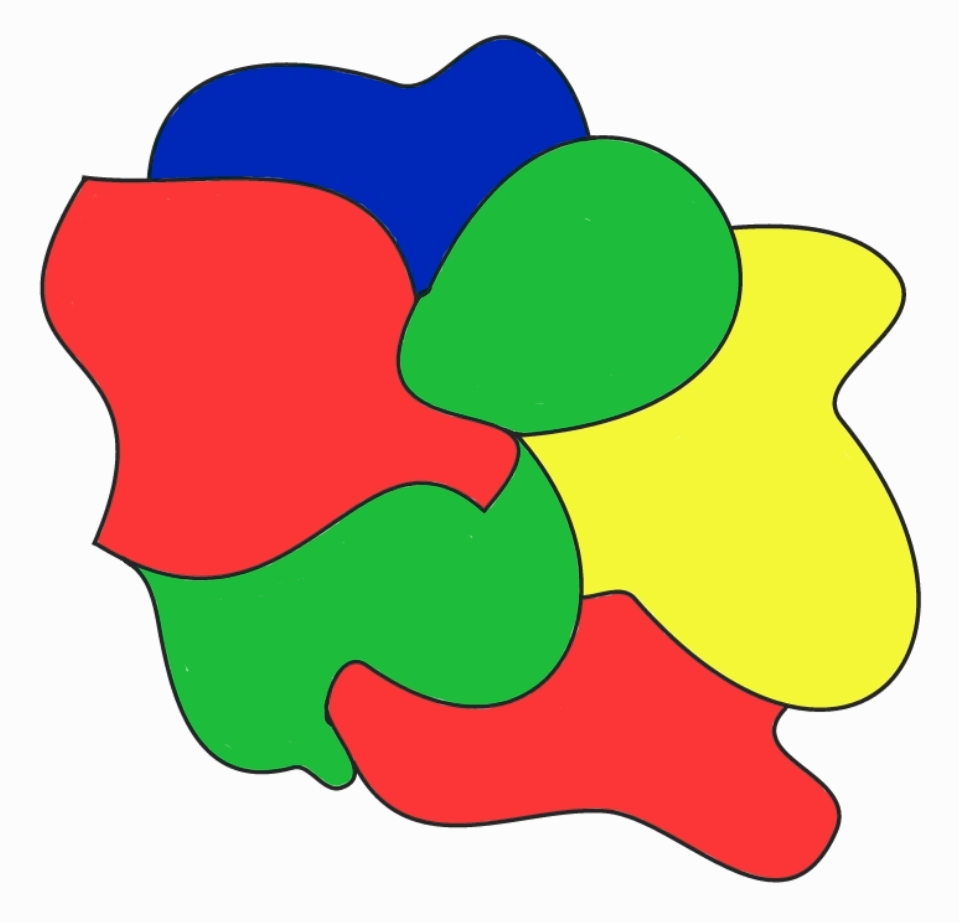
\includegraphics[width=0.5\textwidth]{Mappa.jpg}}; 
			\begin{scope}[x={(image.south east)},y={(image.north west)}]
			    \node[text=white] at (0.4, 0.83) {$R_1$};
			    \node at (0.78, 0.45) {$R_5$};
		    	\node at (0.6, 0.7) {$R_3$};
		    	\node at (0.38, 0.35) {$R_4$};
		    	\node at (0.6, 0.2) {$R_6$};
		    	\node at (0.25,0.6) {$R_2$};
			\end{scope}
		\end{tikzpicture}
		\caption{Esempio di mappa planare $\mathcal{M}$ colorata utilizzando 4 colori.}
		\label{fig:mappa1}
	\end{figure}
	\end{frame}
	
	% Storia del Teorema
	\begin{frame}{Storia del Teorema}
		\begin{itemize}
			\item Origine (1852): Francis Guthrie, intento a colorare una cartina delle contee d'Inghilterra, formula la Congettura dei Quattro Colori.
			\item Dimostrazioni errate di Kempe e Tait (1879-1880): nonostante gli errori pongono le basi per gli sviluppi futuri.
			\item Le dimostrazioni di Appel e Haken (1976) e di Robertson et al. (1996): la prima dimostrazione corretta, ma controversa a causa dell'uso massiccio del computer, e una versione ottimizzata che dissipa quasi tutti i dubbi della comunità matematica, nonostante utilizzi metodi simili.
		\end{itemize}
    \end{frame}

	% Teoria dei Grafi
	\begin{frame}{Definizioni fondamentali}
		Per riformulare il Teorema dei Quattro Colori in funzione di grafi sono necessarie alcune definizioni fondamentali di Teoria dei grafi.
		\begin{itemize}
			\item \emph{Grafo planare}: grafo rappresentabile nel piano senza intersezioni tra gli archi.
		\end{itemize}
		I grafi trattati in questa tesi sono tutti grafi planari.
	\end{frame}
	
	\begin{frame}{Definizioni fondamentali}
		\begin{itemize}
			\item \emph{Colorazione propria}: dato un grafo $G=(V,E)$, una colorazione propria dei vertici di G con k colori è una funzione $c \colon V \to \{1,\dots,k\}$, tale che $\forall u, v \in V$, $c(u) \ne c(v)$ se $(u,v) \in E$.
			\item \emph{Numero cromatico}: denotato con $\chi(G)$, è il numero minimo di colori necessari per ottenere una colorazione propria dei vertici del grafo.
		\end{itemize}
	\end{frame}
	
	\begin{frame}{Definizioni fondamentali}
		\begin{figure}
			\centering
			\begin{tikzpicture}
				
			    \node[circle, draw, fill=blue!70] (a) at (7, 0) {};
			    \node[circle, draw, fill=red!70] (b) at (7.5, 2.5) {};
			    \node[circle, draw, fill=yellow!70] (g) at (8.8, 0.8) {};
			    \node[circle, draw, fill=blue!70] (e) at (10.5, -0.5) {};
			    \node[circle, draw, fill=yellow!70] (f) at (8.5, -1.5) {};
			    \node[circle, draw, fill=red!70] (d) at (12,1.5) {};
			    \node[circle, draw, fill=yellow!70] (c) at (10, 3) {};
			    
			    \draw (a) -- (b) -- (c) -- (d) -- (e) -- (f) -- (a);
			    \draw (a) -- (g) --(b);
			    \draw (c) -- (e);
			    \draw (e) -- (g);
			\end{tikzpicture}
			\vspace{0.5cm}
			\caption{Una 3-colorazione del grafo planare $G$ (infatti $\chi(G) = 3$).}
		\end{figure}
	\end{frame}
	
	\begin{frame}{Riformulazione del Teorema}
		Possiamo allora riformulare il Teorema con riferimento alla colorazione di grafi, nella forma dimostrata nel 1976.
		\vspace{0.3cm}
		\\{\bfseries Teorema dei Quattro Colori (Appel e Haken, 1976).} Dato un grafo planare $G$, $\chi(G) \leq 4$.
	\end{frame}
	
	\begin{frame}{Riformulazione del Teorema}
		\begin{figure}
			\centering
			\begin{tikzpicture}
				\node[anchor=south west, inner sep=0] (image) at (0,0) 
				{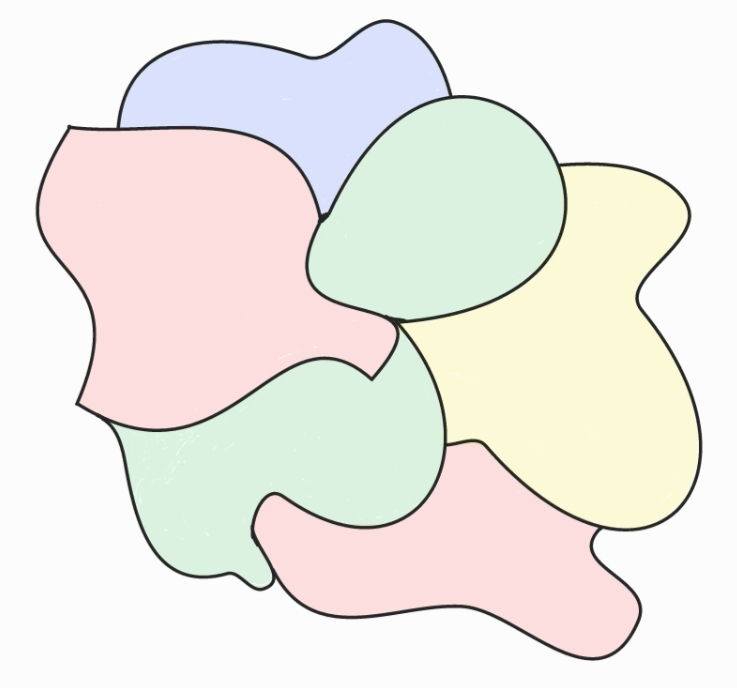
\includegraphics[width=0.5\textwidth]{Mappa2.jpg}}; 
				\begin{scope}[x={(image.south east)},y={(image.north west)}]
					\node[circle, draw, fill=blue] (A) at (0.42,0.82) {};
					\node[circle, draw, fill=red] (B) at (0.31,0.57) {};
					\node[circle, draw, fill=green] (C) at (0.6,0.68) {};
					\node[circle, draw, fill=green] (D) at (0.41,0.34) {};
					\node[circle, draw, fill=yellow] (E) at (0.72,0.45) {};
					\node[circle, draw, fill=red] (F) at (0.63,0.21) {};	
					
					\draw[thick] (B) -- (A) -- (C) -- (B) -- (D) -- (E) -- (F) -- (D);
					\draw[thick] (C) -- (E);
				\end{scope}
			\end{tikzpicture}
			\caption{La mappa $\mathcal{M}$ rappresentata nella Figura~\ref{fig:mappa1} e il grafo corrispondente, con una colorazione propria con 4 colori equivalente.}
			\label{fig:mappa}
		\end{figure}
	\end{frame}
	
	% Dimostrazioni principali
	\begin{frame}{La dimostrazione errata di Kempe}
		Chiariamo con un esempio il concetto, fondamentale nella dimostrazione (errata) di Kempe (1879), di \emph{catena di Kempe}.
		\begin{itemize}
			\item In un grafo $G = (V, E)$ con una colorazione propria dei vertici, una {\bfseries catena di Kempe} rossa-blu che contiene uno specifico vertice rosso si trova individuando tutti i vertici blu ad esso adiacenti, tutti i vertici rossi adiacenti ad ognuno di essi e così via.
		\end{itemize}
	\end{frame}
	
	\begin{frame}{La dimostrazione errata di Kempe}
		\begin{figure}
			\centering
			\begin{tikzpicture}
				\node[circle, draw, fill=blue!60] (a) at (0,0) {};
				\node[circle, draw, fill=red!60] (b) at (1,1) {};
				\node[circle, draw, fill=blue!60] (c) at (2.5,0.5) {};
				\node[circle, draw, fill=red!60] (d) at (0.5,-1) {};
				\node[circle, draw, fill=blue!60] (e) at (3,2) {};
				\node[circle, draw, fill=red!60] (f) at (3.2,-0.5) {};
				\node[circle, draw, fill=blue!60] (g) at (4.2,0.3) {};
				\node[circle, draw, fill=red!60] (h) at (5.2,1.5) {};
				\node[circle, draw, fill=blue!60] (i) at (0.2,2.5) {};
				\node[circle, draw, fill=red!60] (j) at (5,2.3) {};
				
				\draw (d) -- (a) -- (b) -- (c) -- (f) -- (g);
				\draw (e) -- (j);
				\draw (i) -- (b) -- (e) -- (h);
			\end{tikzpicture}
			\vspace{0.5cm}
			\caption{Catena di Kempe rossa-blu. Si tratta di un sottografo di $G$ in cui ogni arco è incidente a un vertice blu e uno rosso.}
		\end{figure}
	\end{frame}
	  
	\begin{frame}{La dimostrazione errata di Kempe}
		\emph{Dimostrazione (con errore).} Induzione sul numero di vertici:
		\begin{itemize}
			\item Sia ogni grafo con $\lvert V \rvert = n$ 4-colorabile, e consideriamo un grafo $G = (V, E)$ con $\lvert V \rvert = n + 1$. Individuiamo un vertice $v \in V$ con $\deg(v) \leq 5$ (si dimostra che è sempre presente) e coloriamo con 4 colori il resto del grafo: è sufficiente colorare $v$ per ottenere una 4-colorazione di $G$.
		\end{itemize}
	\end{frame}
	
	\begin{frame}{La dimostrazione errata di Kempe}
		Consideriamo soltanto il caso in cui $\deg(v) \in \{4, 5\}$: i vertici adiacenti a $v$ possono essere colorati con 4 colori diversi, utilizziamo le catene di Kempe per ridurre il numero dei colori a 3 e risolvere il problema.
		\\Rappresentiamo due esempi esplicativi nel caso in cui $\deg(v) = 4$.
	\end{frame}
	
	\begin{frame}{La dimostrazione errata di Kempe}
		\begin{figure}
			\centering
			\resizebox{\textwidth}{!}{
				\begin{tikzpicture}
					\node[circle, draw] (v) at (0,0) {$v$};
					\node[circle, draw, fill=red!50] (R) at (0.2,1.8) {R};
					\node[circle, draw, fill=yellow!50] (G) at (2.3,0.3) {G};
					\node[circle, draw, fill=green!50] (V) at (0.4,-1.7) {V};
					\node[circle, draw, fill=blue!50] (B) at (-1.7,-0.6) {B};
					\node[circle, draw, fill=yellow!50] (G1) at (-3,0.2) {};
					\node[circle, draw, fill=blue!50] (B1) at (-4,-0.4) {};
					\node[circle, draw, fill=yellow!50] (G2) at (-3.6,-1.8) {};
					\node[circle, draw, fill=blue!50] (B2) at (-2.6,-2.5) {};
					\node[circle, draw, fill=yellow!50] (G3) at (-1.3,-2) {};
					
					\draw (B) -- (v) -- (G);
					\draw (R) -- (v) -- (V);
					\draw (G3) -- (B) -- (G1) -- (B2) -- (G2);
					\draw (G1) -- (B1);
					
					\draw[->, thick] (3.3,0) -- (5.3,0);
					
					\node[circle, draw, fill=blue!50] (v') at (10.3,0) {$v$};
					\node[circle, draw, fill=red!50] (R') at (10.5,1.8) {R};
					\node[circle, draw, fill=yellow!50] (G') at (12.6,0.3) {G};
					\node[circle, draw, fill=green!50] (V') at (10.7,-1.7) {V};
					\node[circle, draw, fill=yellow!50] (B') at (8.6,-0.6) {B};
					\node[circle, draw, fill=blue!50] (G1') at (7.3,0.2) {};
					\node[circle, draw, fill=yellow!50] (B1') at (6.3,-0.4) {};
					\node[circle, draw, fill=blue!50] (G2') at (6.7,-1.8) {};
					\node[circle, draw, fill=yellow!50] (B2') at (7.7,-2.5) {};
					\node[circle, draw, fill=blue!50] (G3') at (9,-2) {};
					
					\draw (B') -- (v') -- (G');
					\draw (R') -- (v') -- (V');
					\draw (G3') -- (B') -- (G1') -- (B2') -- (G2');
					\draw (G1') -- (B1');
				\end{tikzpicture}
			}
			\vspace{-0.3cm}
			\caption{Inversione dei colori nella catena di Kempe blu-gialla contenente B (ma non $G$). In questo modo $v$ può essere colorato di blu.}
		\end{figure}
	\end{frame}
	
	\begin{frame}{La dimostrazione errata di Kempe}
		\begin{figure}
			\centering
			\resizebox{\textwidth}{!}{
			\begin{tikzpicture}
				\node[circle, draw] (v) at (0,0) {$v$};
				\node[circle, draw, fill=red!50] (R) at (0.2,1.8) {R};
				\node[circle, draw, fill=yellow!50] (G) at (2.3,0.3) {G};
				\node[circle, draw, fill=green!50] (V) at (0.4,-1.7) {V};
				\node[circle, draw, fill=blue!50] (B) at (-1.7,-0.6) {B};
				
				\node[circle, draw, fill=green!50] (V1) at (-1.5,2.3) {};
				\node[circle, draw, fill=red!50] (R1) at (-1.2,1.2) {};
				\node[circle, draw, fill=green!50] (V2) at (2.8,1.5) {};
				\node[circle, draw, fill=red!50] (R2) at (1.2,2.8) {};
				
				\draw (B) -- (v) -- (G);
				\draw (R) -- (v) -- (V);
				
				\draw (R1) -- (V1) -- (R2) -- (V2);
				\draw (R) -- (V1);
				
				\draw[line width=2pt, blue] (B) .. controls (-0.3,-2.9) and (1.5,-2.9) .. (G);
				\draw[dashed, line width=2pt, yellow] (B) .. controls (-0.3,-2.9) and (1.5,-2.9) .. (G);
				
				\draw[->, thick] (3.8,0) -- (5.8,0);
				
				\node[circle, draw, fill=red!50] (v') at (8.5,0) {$v$};
				\node[circle, draw, fill=green!50] (R') at (8.7,1.8) {R};
				\node[circle, draw, fill=yellow!50] (G') at (10.8,0.3) {G};
				\node[circle, draw, fill=green!50] (V') at (8.9,-1.7) {V};
				\node[circle, draw, fill=blue!50] (B') at (6.8,-0.6) {B};
				
				\node[circle, draw, fill=red!50] (V1') at (7,2.3) {};
				\node[circle, draw, fill=green!50] (R1') at (7.3,1.2) {};
				\node[circle, draw, fill=red!50] (V2') at (11.3,1.5) {};
				\node[circle, draw, fill=green!50] (R2') at (9.7,2.8) {};
				
				\draw (B') -- (v') -- (G');
				\draw (R') -- (v') -- (V');
				
				\draw (R1') -- (V1') -- (R2') -- (V2');
				\draw (R') -- (V1');
				
				\draw[line width=2pt, blue] (B') .. controls (8.2,-2.9) and (10,-2.9) .. (G');
				\draw[dashed, line width=2pt, yellow] (B') .. controls (8.2,-2.9) and (10,-2.9) .. (G');
			\end{tikzpicture}
		}
			\vspace{-0.7cm}
			\caption{La catena di Kempe blu-gialla contenente $B$ contiene anche $G$ (è ciclica). Inversione dei colori nella catena di Kempe rossa-verde (non ciclica) contenente R. 
			\newline In questo modo $v$ può essere colorato di rosso.}
		\end{figure}
	\end{frame}
	
	\begin{frame}{La dimostrazione errata di Kempe}
	    Se $\deg(v) = 5$ la dimostrazione è più complicata, ma utilizza lo stesso metodo presentato negli esempi. \hspace{3.4cm} $\square$
	    \vspace{0.2cm}
	    \\Tuttavia, proprio in quest'ultimo caso è presente un errore ed esistono controesempi in cui il metodo non è applicabile.
	    \begin{figure}
	    	\centering
	    	\resizebox{0.4\textwidth}{!}{
	    	\begin{tikzpicture}
	    		\node[circle, draw, fill=blue!50] (a) at (0,0) {};
	    		\node[circle, draw, fill=yellow!50] (b) at (-3,-0.9) {};
	    		\node[circle, draw, fill=green!50] (c) at (3,-0.9) {};
	    		\node[circle, draw, fill=green!50] (d) at (-1.2,0.9) {};
	    		\node[circle, draw, fill=yellow!50] (e) at (1.2,0.9) {};
	    		\node[circle, draw, fill=red!50] (f) at (-1.2,1.8) {};
	    		\node[circle, draw, fill=red!50] (g) at (1.2,1.8) {};
	    		\node[circle, draw, fill=blue!50] (h) at (0,2.4) {};
	    		\node[circle, draw] (i) at (0,4.8) {$v$};
	    		\draw (b) -- (i) -- (f) -- (b) -- (d) -- (f) -- (h) -- (i) -- (g) -- (h) -- (d) -- (a) -- (b) -- (c) -- (a) -- (e) -- (g) -- (c) -- (e) -- (h);
	    		\draw (c) -- (i);
	    		\draw (d) -- (e);	
	    		\draw[line width=2pt, blue] (c) -- (a) -- (d) -- (h);
	    		\draw[dashed, line width=2pt, green] (c) -- (a) -- (d) -- (h);
	    		\draw[line width=2pt, blue] (b) -- (a) -- (e) -- (h);
	    		\draw[dashed, line width=2pt, yellow] (b) -- (a) -- (e) -- (h);
	    		\draw[line width=2pt, green] (d) -- (f);
	    		\draw[dashed, line width=2pt, red] (d) -- (f);
	    		\draw[line width=2pt, yellow] (e) -- (g);
	    		\draw[dashed, line width=2pt, red] (e) -- (g);
	    	\end{tikzpicture}
	    }
	    	\caption{Il \emph{grafo di Fritsch}, minimo controesempio alla dimostrazione di Kempe.}
	    \end{figure}
	\end{frame}
	
	\begin{frame}{Il Teorema dei Cinque Colori}
		Nel 1890, Heawood confuta la dimostrazione di Kempe, ma sfrutta anche le stesse tecniche per dimostrare il \emph{Teorema dei Cinque Colori}.
		\vspace{0.3cm}
		\\{\bfseries Teorema dei Cinque Colori (Heawood, 1890).} Dato un grafo planare $G$, $\chi(G) \leq 5$.
	\end{frame}
	
	\begin{frame}{La dimostrazione di Robertson et al.}
		La dimostrazione del Teorema dei Quattro Colori di Robertson, Sanders, Seymour e Thomas (1996) si basa sui metodi utilizzati da Appel e Haken, ma è ottimizzata e semplificata rispetto a quella precedente:
		\begin{itemize}
			\item il numero di \emph{buone configurazioni} e di \emph{regole di scarica} viene ridotto
			\item due programmi indipendenti verificano le dimostrazioni affidate al computer per garantirne la correttezza
			\item l'algoritmo per la 4-colorazione richiede un tempo quadratico e non più di ordine quarto.
		\end{itemize}
	\end{frame}
	
	\begin{frame}{La dimostrazione in breve}
		La dimostrazione non è diretta, come quella di Kempe, ma per contraddizione: si suppone che esista un controesempio al Teorema dei Quattro Colori, in particolare un controesempio minimo, se ne individuano una serie di proprietà e si sfruttano per giungere a una contraddizione.
		\vspace{0.3cm}
		\begin{itemize}
		    \item Un \emph{minimo controesempio} al Teorema dei Quattro Colori è un grafo planare $G$ tale che $\chi(G) = 5$ e, dato un altro grafo $G'$ con $\chi(G') = 5$, $\lvert V(G) \rvert + \lvert E(G) \rvert \leq \lvert V(G') \rvert + \lvert E(G') \rvert$.
		\end{itemize}
	\end{frame}
	
	\begin{frame}{La dimostrazione in breve}
		In particolare la dimostrazione si ottiene provando 3 teoremi:
		\vspace{0.3cm}
		\\{\bfseries Teorema 1.} Ogni minimo controesempio al Teorema dei Quattro colori è una \emph{triangolazione 6-connessa internamente}.
		\\{\bfseries Teorema 2.} Nessun minimo controesempio contiene una \emph{buona configurazione}.
		\\{\bfseries Teorema 3.} Ogni \emph{triangolazione 6-connessa internamente} contiene una \emph{buona configurazione}.
		\vspace{0.3cm}
		\\Se il Teorema 1 è vero, allora i Teoremi 2 e 3 non possono essere contemporaneamente veri.
	\end{frame}
	
	\begin{frame}{Triangolazioni e configurazioni}
		Diamo alcune definizioni.
		\begin{itemize}
		\item Una \emph{triangolazione} è un grafo planare in cui ogni faccia è delimitata da 3 archi.
		\item Un grafo $G$ si dice \emph{6-connesso internamente} se è connesso (esiste un cammino che collega ogni coppia di vertici), ha almeno 6 vertici e, dato un insieme di vertici $X$ tale che $G \smallsetminus X$ non è connesso, $\lvert X \rvert \geq 6$ oppure $\lvert X \rvert = 5$ e $G \smallsetminus X$ ha esattamente due componenti connesse, di cui una costituita da un solo vertice.
	\end{itemize}
	\end{frame}
	
	\begin{frame}{Triangolazioni e configurazioni}
	\begin{figure}
		\centering
		\begin{tikzpicture}[scale=0.8]
			\node[circle, draw, fill=blue] (a) at (0,0) {};
			\node[circle, draw, fill=blue] (b) at (6,0) {};
			\node[circle, draw, fill=blue] (c) at (3,5) {};
			\node[circle, draw, fill=blue] (d) at (2.2,1.6) {};
			\node[circle, draw, fill=blue] (e) at (3.4,2.7) {};
			\node[circle, draw, fill=blue] (f) at (3.3,1) {};
			
			\draw (a) -- (b) -- (c) -- (a) -- (d) -- (c) -- (e) -- (b) -- (f) -- (a);
			\draw (d) -- (e) -- (f) -- (d);
		\end{tikzpicture}
		\vspace{0.5cm}
		\caption{Esempio di triangolazione: ogni faccia è delimitata esattamente da 3 archi (anche la faccia illimitata).}
	\end{figure}
	\end{frame}
	
	\begin{frame}{Triangolazioni e configurazioni}
		Si dimostra che ogni minimo controesempio, se esiste, deve essere una triangolazione.
		\\Inoltre è noto dal 1913 che deve essere anche 6-connesso internamente.
		\vspace{0.3cm}
		\\Vediamo ad esempio perché un minimo controesempio non può avere un separatore $X$ con $\lvert X \rvert = 3$.
	\end{frame}
	
	\begin{frame}{Triangolazioni e configurazioni}
		\begin{figure}
			\centering
			\begin{tikzpicture}[scale=0.4]
				\node[circle, draw, fill=red] (a) at (0,0) {};
				\node[circle, draw, fill=red] (b) at (6,0) {};
				\node[circle, draw, fill=red] (c) at (3,5) {};
				\node[circle, draw, fill=black] (d) at (2.2,1.6) {};
				\node[circle, draw, fill=black] (e) at (3.4,2.7) {};
				\node[circle, draw, fill=black] (f) at (3.8,1) {};
				\node[circle, draw, fill=black] (g) at (3,-1) {};
				\node[circle, draw, fill=black] (h) at (0.64,3.01) {};
				\node[circle, draw, fill=black] (i) at (5.36,3.01) {};
				\node[circle, draw, fill=black] (j) at (3,8) {};
				\node[circle, draw, fill=black] (k) at (-4,-2) {};
				\node[circle, draw, fill=black] (l) at (10,-2) {};
				
				\draw[red, thick] (a) -- (b) -- (c) -- (a);
				\draw (a) -- (d) -- (c) -- (e) -- (b) -- (f) -- (a);
				\draw (d) -- (e) -- (f) -- (d);
				\draw (k) -- (l) -- (j) -- (k) -- (a) -- (h) -- (c) -- (j) -- (h) -- (k) -- (g) -- (l) -- (i) -- (j);
				\draw (a) -- (g) -- (b) -- (i) -- (c);
				\draw (b) -- (l);
			\end{tikzpicture}
			\vspace{0.5cm}
			\caption{$X$, in rosso, è separatore. Le due componenti connesse, in nero, sono 4-colorabili e inducono una colorazione di $X$ sostanzialmente unica. Quindi, l'intero grafo è 4-colorabile.}
		\end{figure}
	\end{frame}
	
	\begin{frame}{Triangolazioni e configurazioni}
		Anche nei casi in cui $\lvert X \rvert = 4,5$ si utilizzano argomenti simili e si giunge quindi alla dimostrazione del Teorema 1.
		\vspace{0.3cm}
	    \\{\bfseries Teorema 1 (Birkhoff, 1913).} Ogni minimo controesempio al Teorema dei Quattro colori è una \emph{triangolazione 6-connessa internamente}.
    \end{frame}

	\begin{frame}{Triangolazioni e configurazioni}
		Per dimostrare i due Teoremi successivi è fondamentale il concetto di \emph{configurazione}.
		\begin{itemize}
		    \item Una \emph{configurazione} $K$ è costituita da una quasi-triangolazione $G(K)$ e una funzione $\gamma_K \colon V(K) \to \mathbb{Z}$ che assegna ad ogni vertice $v \in V(K)$ un valore $\gamma_K(v) \geq \deg(v)$, rispettando una serie di proprietà.
		\end{itemize}
	\end{frame}
	
	\begin{frame}
		\begin{figure}
			\centering
			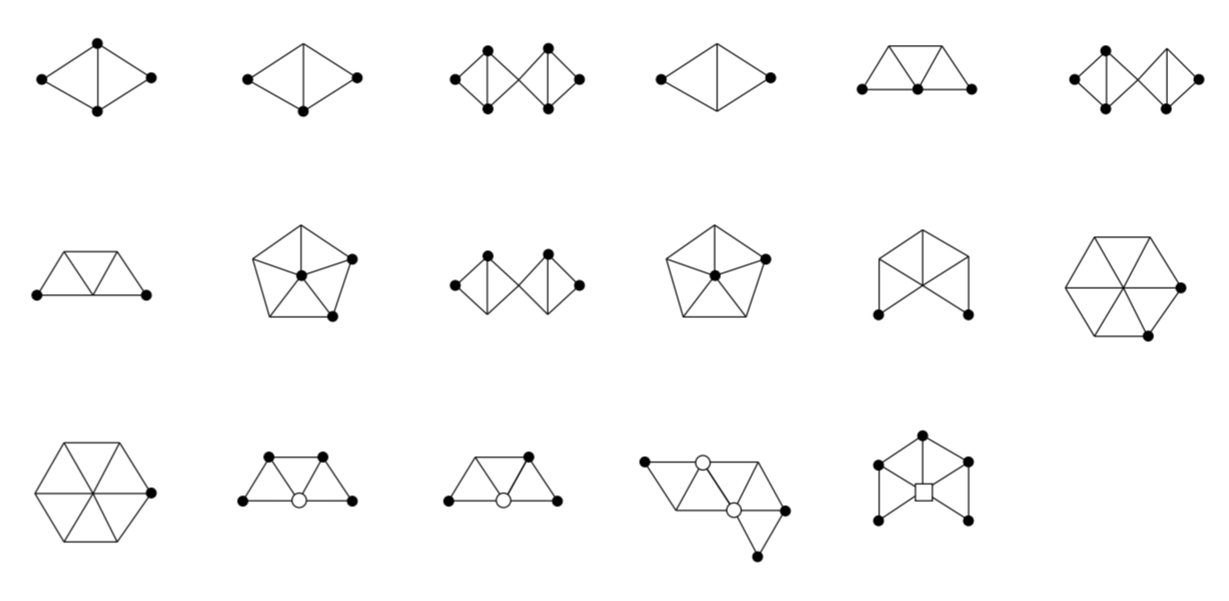
\includegraphics[width=\textwidth]{Immagine1.jpg}
			\caption{Alcune tra le 633 \emph{buone configurazioni} di Robertson et al. \newline I simboli che rappresentano i vertici indicano il valore di $\gamma_K(v)$: \newline
			$\bullet$ se $\gamma_K(v) = 5$, $\cdot$ se $\gamma_K(v) = 6$, $\circ$ se $\gamma_K(v) = 7$ e $\square$ se $\gamma_K(v) = 8$}
			\label{fig:configurazioni}
		\end{figure}
	\end{frame}
	
	\begin{frame}{Riducibilità}
		\begin{itemize}
			\item Una configurazione contenuta in un grafo si dice \emph{riducibile} se è possibile sostituirla con un grafo più piccolo senza sostanzialmente modificare la colorazione dei vertici ad essa adiacenti.
		\end{itemize}
		Si dimostra il seguente Lemma.
		\vspace{0.3cm}
		\\{\bfseries Lemma.} Le 633 \emph{buone configurazioni} sono riducibili.
		\vspace{0.3cm}
		\\Di conseguenza, è verificato anche il Teorema 2.
		\vspace{0.3cm}
		\\{\bfseries Teorema 2.} Nessun minimo controesempio contiene una \emph{buona configurazione}.
	\end{frame}
	
	\begin{frame}{Inevitabilità}
		\begin{figure}
			\centering
			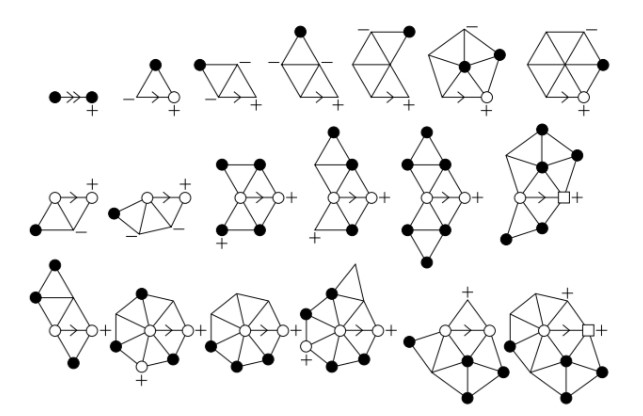
\includegraphics[width=\textwidth]{Regole.jpg}
			\caption{Alcune tra le 32 regole di scarica di Robertson et al.}
			\label{fig:regole}
		\end{figure}
	\end{frame}
	
	\begin{frame}{Inevitabilità}
	    \begin{itemize}
	    	\item Si definisce la carica di un vertice $v$ in funzione del valore di $\deg(v)$ e delle caratteristiche delle regole che contengono $v$.
	    \end{itemize}
	    Si dimostra il seguente Lemma.
	    \vspace{0.3cm}
	    \\{\bfseries Lemma.} Per ogni triangolazione $T$, $\sum_{v \in V(T)} \Theta_T(v) = 120$.
	    \\Perciò, esiste un vertice $v$ di $T$ tale che $\Theta_T(v) > 0$.
	\end{frame}
	
	\begin{frame}{Inevitabilità}
		\textbf{Teorema.} Se $v$ è un vertice di una triangolazione $T$ 6-connessa internamente con $\Theta_T(v) > 0$, allora è presente una buona configurazione contenuta in $T$ in un raggio di due vertici di distanza da $v$.
		\vspace{0.3cm}
		\\La dimostrazione si ottiene sfruttando la geometria delle buone configurazioni e delle regole di scarica e garantisce anche la correttezza del Teorema 3.
		\vspace{0.3cm}
		\\{\bfseries Teorema 3.} Ogni \emph{triangolazione 6-connessa internamente} contiene una \emph{buona configurazione}.
	\end{frame}
	
	\begin{frame}{Conclusioni}
	    L'importanza del Teorema dei Quattro Colori non è soltanto nel risultato in sé, ma anche e soprattutto nell'aver evidenziato quanto la matematica sia strettamente correlata ad ogni altro campo nel mondo della scienza, come in questo caso l'informatica e la programmazione, in continua evoluzione e volta a una comprensione sempre più profonda del mondo che ci circonda.
		
	\end{frame}
	\end{document}
